\chapter{Algoritmus Trooper}

V tejto práci naväzujeme a ďalej vylepšujeme algoritmus Trooper, ktorý bol vytvorený v rámci mojej  bakalárskej práce na Matematicko-Fyzikálnej fakulte \cite{bc}. Preto v tejto kapitole uvedieme princípy fungovania a stav implementácie algoritmu tak, ako bol popísaný v bakalárskej práci.
Jedná sa o algoritmus založený na princípe homológneho modelovania, čo znamená, že predikujeme terciárnu RNA štruktúru na základe primárnej sekvencie molekuly označovanej ako target a známej terciárnej štruktúry a sekvencie inej RNA molekuly označovanej ako template.


\section{Kostra algoritmu}

V nasledujúcom zozname uvázdame postupnosť hlavných krokov algoritmu.\label{3-kostra}
\begin{enumerate}
\item Predpríprava a validácia vstupných súborov: template sekvencia, target sekvencia a štruktúra.
\item Alignemnt: Zarovnanie target a template sekvencií.
\item Sliding window: Algoritmus posuvného okienka na zarovnaní.
\item Treating indels: Vyriešenie medzier v zarovnaní. \label{3-indels}
\item Kopírovanie a mapovanie konzervovaných nukleotidov z target štruktúry do predikovanej template štruktúry. \label{3-map}
\item Vyčlenenie predikcie príliš dlhých medzier v target štruktúre.\label{3-sphere}
\item Príprava vstupu pre FARFAR.
\item Predikcia nekonzervovaných úsekov pomocou algoritmu FARFAR.
\item Zloženie predikovaných úsekov a dlhých medzier do finálnej štruktúry.
\end{enumerate}

\section{Popis algoritmu}
Ako vstup algoritmus dostane target sekvenciu a template sekvenciu aj štruktúru. Na výstupe očakávame terciárnu štruktúru target molekuly RNA.


\indent  Ako prvý krok algoritmus skontroluje, či sú sekvencia vo fasta súbore a štruktúra v pdb súbore rovnako indexované. Nukleotidy v pdb súbore sú očíslované, ale vo fasta súbore číslo nukleotidu odpovedá jeho pozícii v súbore. Kontrolujeme to prechodom cez pdb súbor tak, že indexom nukleotidu z pdb zaindexujeme do fasta súboru a typ nukleotidu musí byť v oboch súboroch na tejto pozícii zhodný. V prípade, že zhodný nie je, skúšame ešte posunúť fasta sekvenciu pridaním dummy nukleotidov na začiatok sekvencie (pre prípad, že by začiatok sekvencie v súbore chýbal). Ak sa nám nepodarí ani takýmto spôsobom dosiahnuť, aby sa typy nukleotidov v rovnakých indexoch zhodovali, označíme target za nevhodný pre predikciu a algoritmus končí neúspechom.


\indent V druhom kroku urobíme globálne zarovnanie (alignment) target a template sekvencií v programe Emboss Needle. Na vytvorené zarovnanie použijeme algoritmus posuvného okienka (sliding window) a pre každú pozíciu určíme percentuálnu mieru okolitých úspešne zarovnaných nukleotidov spadajúcich do okienka. V prípade, že získaná hodnota je vyššia ako parametrom určená hranica, označíme príslušnú pozíciu v zarovnaní ako konzervovanú. 


\indent V treťom kroku sa zaoberáme medzerami (indels), ktoré vznikli v terget alebo template sekvencii pri zarovnaní. Inak povedané, do oboch sekvencií mohol algoritmus zarovnania ľubovoľne vložiť medzery alebo na seba zarovnať nezhodujúce sa nukleotidy tak, aby získal zarovnanie s čo najlepším skóre \autoref{tab3.1}. 
To znamená, že medzery v inak konzervovanom úseku template sekvencie by vo výsledku nenechali miesto na doplnenie nukleotidov z target sekvencie zarovnaných oproti týmto medzerám z template sekvencie. 
Naopak, medzery v target sekvencii zarovnané oproti nukleotidom v template sekvencii v inak konzervovanom úseku by mohli spôsobiť medzeru v predikovanej štruktúre, nakoľko by sme z fragmentu konzervovanej štruktúry len odmazali nejaké nukleotidy a ničím ich nedoplnili. \autoref{obr3.1:indels}
Oba tieto problémy riešime tak, že nukleotidy v určitom okolí takýchto úsekov označíme za nekonzervované a budú dopredikované algoritmom FARFAR.
Taktiež označíme za nekonzervované tie nukleotidy, ktoré boli zarovnané na nezhodujúci sa typ nukleotidu. 

\begin{table}[b!]
\centering
\begin{tabular}{ccccc}
\toprule
Sekvencia  & konzervované  & nekonzervované & gap & gap \\
\midrule
tamplate  & G  & A & - & U \\
target  & G  & G & C & - \\
\bottomrule
\end{tabular}
\caption{Prehľad štyroch situácií, ktoré môžu nastať na každej pozícii v zarovnaní dvoch sekvencií.}\label{tab3.1}
\end{table}

\begin{figure}%[p]\centering
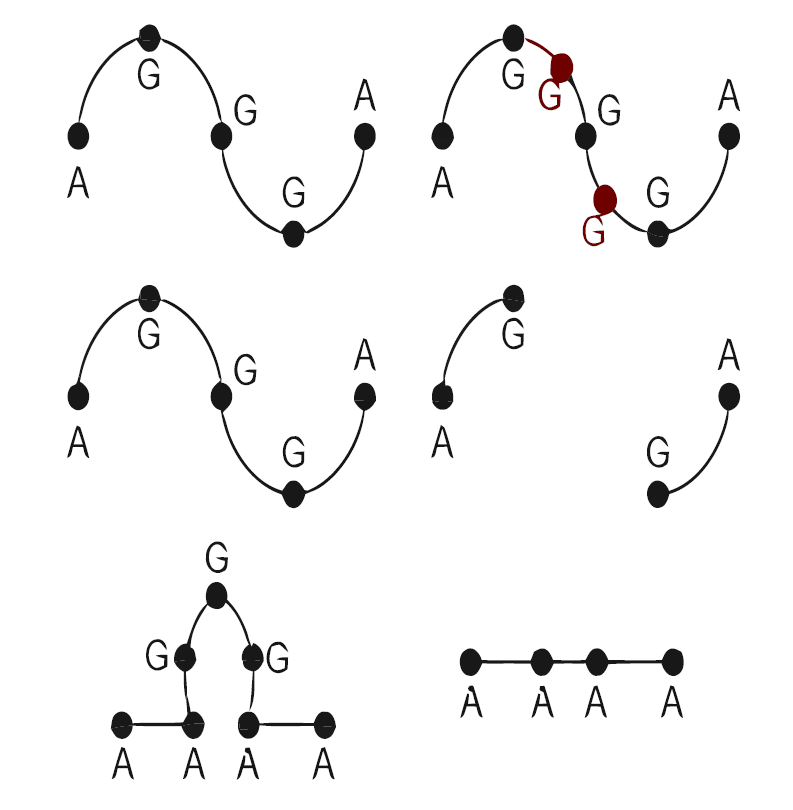
\includegraphics[width=\textwidth]{../img/aln-problems}
\caption{Problémy, ktoré môžu nasať v štruktúre pri vložení medzier do target alebo template časti zarovnania. Prvý riadok zobrazuje komplikácie pri pokuse vložiť nukleotidy (znázornene červenou farbou) do celistvej štruktúry (teda v zarovnaní boli pridané medzery do target sekvencie). Druhý riadok ukazuje opačný problém, a to vynechanie dvoch nukleotidov a roztrhnutie štruktúry (zodpovedá to vložením medzier do target sekvencie). Tretí riadok odpovedá rovnakej situácii ako druhý, ale odstránenie nukleotidov zo štruktúry nespôsobuje problém, pretože odstránené nukleotidy tvorili loop, ktorý môžeme bez problémov odobrať.}
\label{obr3.1:indels}
\end{figure}



\indent V štvrtom kroku skopírujeme konzervované časti template štruktúry do predikovanej target štruktúry. Vzhľadom na to, že v zarovnaní môžu byť rôzne vložené medzery do target aj template sekvencie, musíme premapovať indexy nukleotidov z template štruktúry tak, aby odpovedali nukleotidom, na ktorých miesto sú vložené v target sekvencii. Toto urobíme jednoducho vďaka informáciám zo zarovnania. Takto získame target štruktúru s medzerami, ktoré potrebujeme dopredikovať.


\indent V piatom kroku identifikujeme dlhé nekonzervované úseky a vyčleníme ich následnu predikciu do samostatných behov algoritmu FARFAR. 
Prvým dôvodom je, že takto sa môže FARFAR zamerať iba na predikciu dlhého úseku, a tým znížime celkovú výpočetnú náročnosť. Takisto môžeme zmeniť jeho parametry, ako napríklad zvýšiť počet samplovaných modelov, prípade zvýšiť celkový čas predikcie. 
Ďalším dôvodom, prečo dopredikovanie nekonzervovaných úsekov takto delíme je, že algoritmus FARFAR sa nedokáže dobre vysporiadať s predikciami príliš dlhých štruktúr, aj keď je časť nukleotidov pevne daná. Z tohto dôvodu rozdeľujeme dlhé štruktúry na úseky dĺžky 300 nukleotidov na základe ich poradia v sekvencii. Takéto delenie spôsobuje ďalší problém - nukleotidy, ktoré sú od seba vzdialené v sekvencii môžu byť blízko pri sebe v terciárnej štruktúre. 
Naše riešenie teda vyberie tieto dlhé nekonzervované úseky spolu s okolitými nukleotidmi, ktoré ležia v guli so stredom určeným úsečkou spájajúcou posledný konzervovaný nukleotid pred nekonzervovaným úsekom s prvým konzervovaným nukleotidom za nekonzervovaným úsekom vzhľadom na ich poradie v sekvencii. Polomer tejto gule je určený empiricky ako 0,75-násobok dĺžky úsečky, kedy by guľa mala obsiahnuť všetky relevantné nukleotidy. \autoref{obr3.2:sphere}

\begin{figure}%[p]\centering
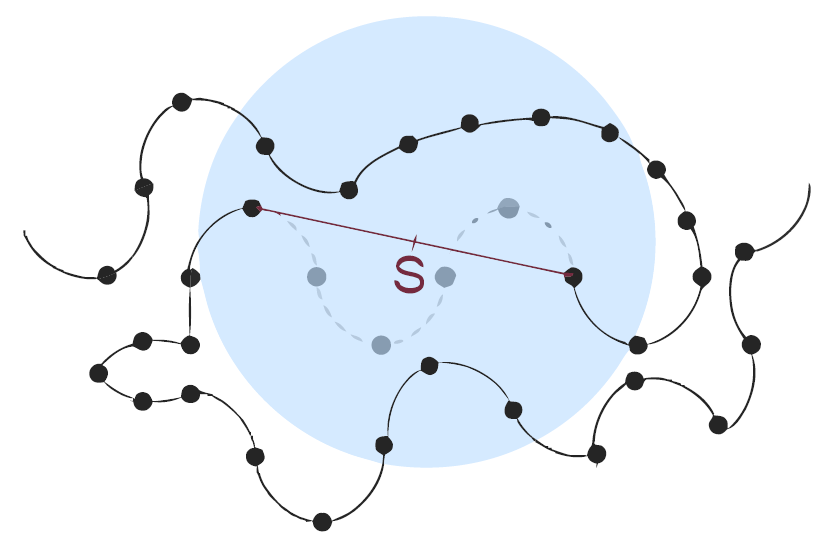
\includegraphics[width=\textwidth]{../img/sphere}
\caption{Schématické nakreslenie sféry so stredom v bode S, ktorý je stredom úsečky spájajúcej dva krajné konzervované nukleotidy medzery v štruktúre. Všetky nukleotidy, ktoré padnú do bledomodrej gule, budú použíte pri predikcii daného úseku.}
\label{obr3.2:sphere}
\end{figure}

\indent V šiestom kroku pripravíme vstupné dáta pre algoritmus FARFAR. To zahŕňa prípadné rozdelenie na úseky po 300 nukleotidov spomenuté v predchádzajúcom odstavci a prepísanie informácií o tom, ktoré nukleotidy sú pevne dané a ktoré treba dopredikovať do vstupného súboru. Takisto tu určíme parametre pre jednotlivé predikcie, ako napríklad počet vygenerovaných štruktúr.  


\indent
V siedmom kroku všetky takto pripravené časti predikcie spustíme a počkáme na výsledok. Toto je najpomalšia časť algoritmu, kedy FARFAR potrebuje čas minimálne pár hodín až niekoľko desiatok hodín, aby dokázal predikovať dlhšie nekonzervované úseky. Tie sú napriek tomu najväčšou slabinou nášho algoritmu, pretože podľa výsledkov získaných v bakalárskej práci platí, že čím dlhšie nekonzervované úseky sa nachádzajú v predikovaných štruktúrach tým je presnosť predikcie nižšia.


\indent V poslednom kroku najprv konvertujeme úseky z internej reprezentácie FARFARu do klasických pdb súborov a tie spojíme do výsledku.  


\section{Používané typy súborov}
V algoritme opakovane pracujeme s určitými typmi textových súborov. Sú to súbory s príponami fasta \textit{(uloženie sekvencie)}, secstr \textit{(uloženie sekundárnej štruktúry)}, pdb \textit{(uloženie terciárnej štruktúry)} a aln \textit{(uloženie zarovnania dvoch sekvencii)} \autoref{obr3.25:files}.

\begin{figure}%[p]\centering
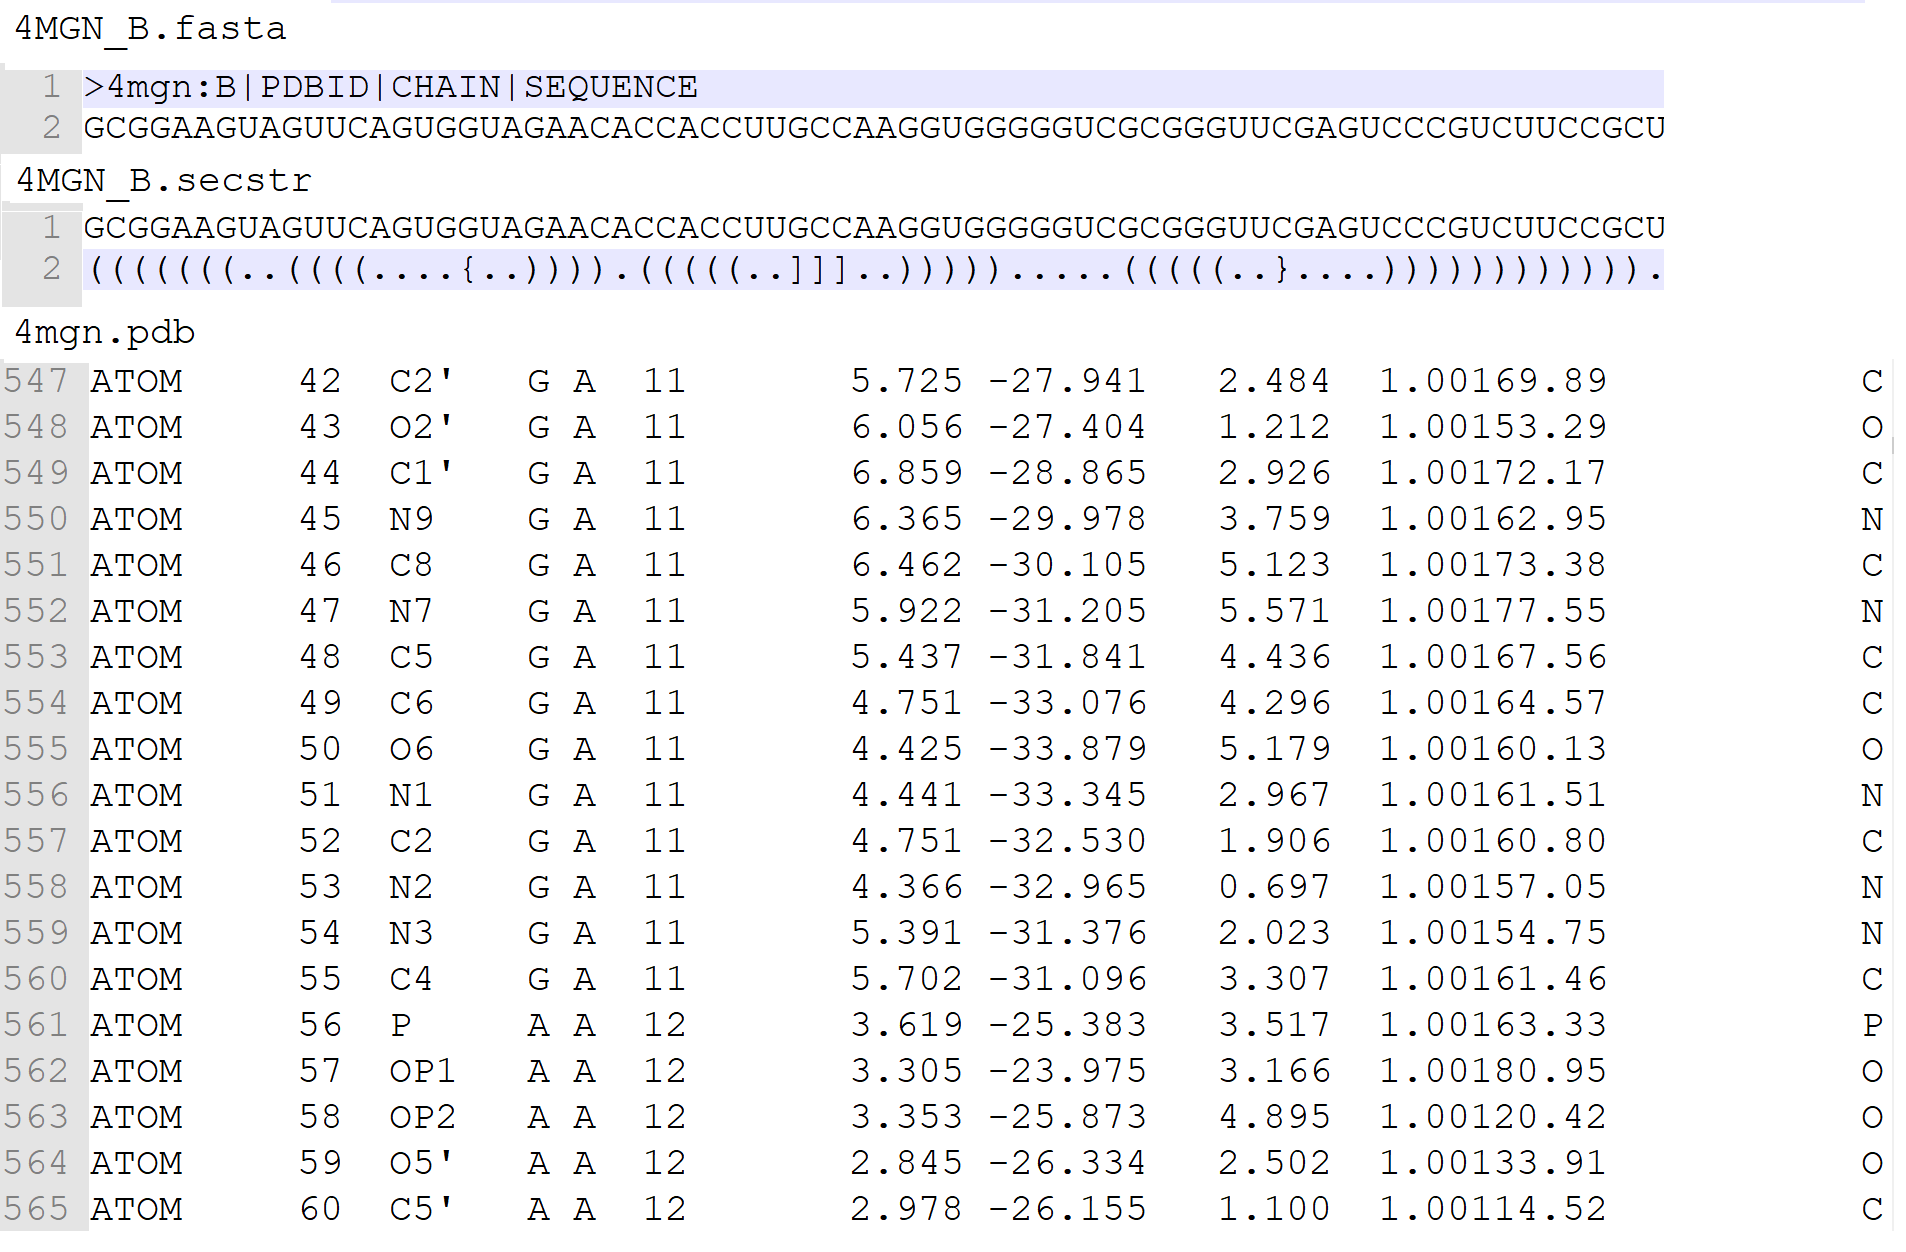
\includegraphics[width=\textwidth]{../img/files}
\caption{Na obrázku vidíme zhora nadol príklady súborov fasta, secstr a pdb pre molekulu 4mgn.}
\label{obr3.25:files}
\end{figure}

\indent Súbory typu fasta slúžia na ukladanie sekvencií. Pozostávajú z dvoch riadkov, v prvom je identifikátor sekvencie pozostávajúci z jej názvu a chain-u (jedna sekvencia máva  často viacero chains) a v ďalších riadkoch sú za sebou zoradené jednotlivé nukleotidy \textit{A, C, G, U}. V prípade, že je nejaký nukleotid v rade neznámy, bežne sa namiesto jeho typu úvádza písmeno \textit{N} alebo \textit{X}.


 \indent Súbory secstr nám slúžia na ukladanie informácií o sekundárnej štruktúre molekuly. Sú tvorené kombináciou rôznych typov zátvoriek, ktoré popisujú sekundárnu štruktúru tak, že medzi nukleotidmi odpovedajúcimi zátvorkám existuje chemická väzba - takéto dva nukleotidy sa tiež nazývajú base pair. Z toho vyplýva, že sa v terciárnej štruktúre budú nachádzať blízko pri sebe. Bodka v sekundárnej štruktúre znamená, že nukleotid netvorí base pair so žiadnym ďalším nukleotidom. Rôzne typy zátvoriek  ako \textit{[] , \{\}, <>} reprezentujú pseudouzly \cite{dbnotation}.


\indent Súbory typu pdb uchovávajú okrem iného informácie o jednotlivých atómoch molekuly. V každom riadku sú uložené informácie o presných koordinátoch atómu v 3D priestore, typ atómu vrámci nukleotidu, chain do ktorej atóm patrí a index nukleotidu, ktorému patrí. PDB súbory často nie sú kompletné, chýbajú v nich atómy alebo celé nukleotidy. Takisto sa stáva, že indexy nukleotidov v pdb súboroch a fasta súboroch nesúhlasia. Táto nekonzistentnosť medzi súbormi, alebo chýbajúce časti pdb súborov sťažujú ich algoritmické spracovanie.


\indent Súbory s príponou aln označujú výstup zarovnania dvoch sekvencií z programu EMBOSS Needle. Súbor obsahuje presné zarovnanie sekvenciií, skóre zarovnania, percentuálny pomer medzier v zarovnaní (gaps) a percentuálny pomer korektne zarovnaných nukleotidov označený ako similarity. 


\section{Popis implementácie}
Algoritmus bol implementovaný prevažne v programovacom jazyku Python 2.7. s využitím knižnice BioPython, ktorá zjednodušuje prácu so štandardnými súbormi používanými v bioinformatike, ako napríklad pdb a fasta. Okrem toho sme použili bash scripty na manipuláciu so súbormi a spustenie predikcie vo FARFAR.


\indent Algoritmus bol rozdelený na tri časti. Prvá pozostávala zo spustenia predikcie dopredu pripravenej target-template dvojice molekúl na lokálnom PC s operačným systémom Windows. To obsiahlo algoritmus  po siedmy krok, teda bola pipravená target štruktúra do stavu, kedy treba dopredikovať nekonzervované úseky algoritmom FARFAR. Následne boli takto pripravené vstupy pre FARFAR skopírované na servery organizácie Metacentrum používajúce operačný systém unixového typu s dávkovým spracovaním úloh. Vďaka tomu, že predikcie nekonzervovaných úsekov v rámci jednej molekuly sú na sebe nezávislé a tiež predikcie molekul medzi sebou sú nezávislé, môžeme predikcie nekonzervovaných úsekov algoritmom FARFAR paralelizovať. To je veľmi dôležité, pretože de novo predikcia nekonzervovaných úsekov bola najdlhšie trvajúca časť algoritmu a predikcia jednej štruktúry mohla obsahovať niekoľko takýchto de novo predikcií.  Po skončení FARFAR predikcií nekonzervovaných úsekov boli výsledky skopírované späť na lokálny PC a tam boli v treťom kroku vyhodnotené výsledky. 


\indent Časová náročnosť celého algoritmu je závislá hlavne na nekonzevovaných úsekoch, ktoré treba predikovať. Časť predikcie po algoritmus FARFAR beží v rádoch desiatok sekúnd. Pre FARFAR sme okrem pár problémových predikcií používali obmedzenie predikcie časom 24 hodín, prípadne 100 štruktúr. To znamená, že FARFAR buď stihne do 24 hodín namodelovať 100 modelov štruktúr, alebo s modelovaním skončí predčasne po 24 hodinách a výsledkom bude počet modelov štruktúr, ktoré sa mu do 24 hodín podarilo namodelovať. Z namodelovaných štruktúr sa vyberie tá s najmenšou voľnou energiou. Počet a kvalita kandidátskych štruktúr, ktoré za tento čas algoritmus stihne vygenerovať, záleží na počte nekonzervovaných úsekov, ich dĺžke (problematické sú hlavne dlhé nekonzervované úseky) a dĺžke celej predikovanej štruktúry včetne konzervovaných nukleotidov. Záverečné získanie výsledkov a porovnanie s experimentálne získanými štruktúrami prebieha opäť v rádoch desiatok sekúnd.


\section{Pseudokód}\label{kap3:pseudocode}
V tejto sekcii uvádzame pseudokód algoritmu Trooper v stave po bakalárskej práci. Premenné  začínajú malým písmenom, názvy metód veľkým písmenom. Pseudokód ignoruje prácu s datami a znaky \textit{[]} za premennou znamenajú, že premenná nahrádza množinu pdb súborov. Pseudokód nám bude ďalej v práci slúžiť aj na to, aby sme sa vedeli na jendotlivé metódy v prípade potreby odkazovať.


\lstset{numbers=left, numberstyle=\tiny, stepnumber=1, numbersep=5pt}
\begin{lstlisting}
Main(fastaTarget, fastaTemplate, pdbTemplate)
{
   CheckTemplateMapping
      (fastaTemplate, pdbTemplate)
   alignment := Align
      (fastaTarget, fastaTemplate)
   alignment1 := UseSlidingWindow
      (alignment)
   alignment2 := ProcessGaps
      (alignment1)
   conservedParts := CopyConservedParts
      (alignment2, pdbTemplate)
   mappedConservedParts := MapConservedParts
      (conservedParts, alignment2)
   longParts[] := ProcessLongUnconservedParts
      (mappedConservedParts)
   shortParts[] := ProcessShortUnconservedParts
      (mappedConservedParts)
   predictedParts[] := PredictUnconservedParts
      (longParts[], shortParts[])
   finalModel := ConnectPredictedParts
      (predictedParts)
}

CheckTemplateMapping(fasta, pdb)
{
   foreach res in pdb
   {
         if (fasta[res[id]] != res[type])
         ERROR: Input needs manual editing!
         EXIT PROGRAM	
   }
}

Align(fastaTarget, fastaTemplate)
{
   string alignment := CallEmbossAln
      (fastaTarget, fastaTemplate)
   return EditAlignmentFormat(alignment)
}

SlidingWindow(alignment, windowLength, minimalLimit)
{
   hL = windowLength DIV 2	
   foreach nucleotide in alignment 
   {
      check if in [nucleotide[id]-hL, nucleotide[id]+hL]
      is less than minimalLimit conserved nucleotides
      if so mark nucleotide as unconserved
   }		
   return modifiedAln  
}

ProcessGaps(alignment, cutoff)
{
   foreach gap in alignment 
   {
      alignment := mark "cutoff" nucleotides from 
         both sides of the gap as unconserved 
   }	
   return alignment
}

CopyConservedParts(alignment, pdb)
{
   conservedParts = ""
   foreach nucleotide in pdb 
   {
      if (IsConserved(nucleotide, alignment))
         conservedParts += nucleotide
   }
   return conservedParts
}

MapConservedParts(conservedParts, alignment)
{
   map nucleotide id's from current state (nc with
   id x corresponds to x-th nc in template fasta) to 
   state where nc id correctly corresponds to 
   nucleotide in target fasta 
   return modifiedConservedParts
}

ProcessLongUnconservedParts
   (conservedParts, ncAvarageLength, minLengthGapLimit)
{
   longParts = []
   foreach gap in conservedParts
   {
      if length(gap) <= minLengthGapLimit
         continue
      startNc := conserved nucleotide before gap
      endNc := conserved nucleotide after gap
      ph="phosphor"
      s := FindMiddle(startRes[ph], endRes[ph])
      p := length(gap) * ncAvarageLength / 2
      ncsInSphere := all nucleotides inside sphere(p, s)
      preparedPart := PrepareCorectFormatForFARFAR
         (ncsInSphere)
      longParts[] += preparedPart
   }
   return longParts[]
}

ProcessShortUnconservedParts
   (conservedParts, lengthOfSection, maxLengthGapLimit)
{
   createdSections = []
   createdSections[] = divide "conservedParts" into 
      sections with length of "lengthOfSection"
   preparedSections = []
   foreach section in createdSections[]
   {
      preparedSections[] += PrepareCorectFormatForFARFAR
         (section, maxLengthGapLimit)
   }
   return preparedSections[]
}

PredictUnconservedParts(lgUnconsPts[], shUnconsPts[])
{
   predictedParts = []
   allParts := lgUnconsPts[] + shUnconsPts[]
   foreach input in allParts
   {
      predictedParts[] += CallFARFAR(input)
   }
   return predictedParts[]	
}

ConnectPredictedParts(predictedParts[])
{
   connect all conserved and predicted nucleotides 
   into single file in case of duplicity
   (they are almost the same) choose only one 
}
\end{lstlisting}


\section{Časová zložitosť}
V tejto sekcii rozoberieme časovú zložitosť algoritmu ako reálnu, tak aj asymptotickú, ktorou sme sa v bakalárskej práci nezaoberali. Budeme na to potrebovať definovať premennú dĺžka molekuly \textit{l}, kedy budeme predpokladať, že všetky molekuly s ktorými pracujeme majú takúto dĺžku. 


\indent Asymtoticky zložitosť rozoberieme podľa jednotlivých metód pseudokódu:
 \begin{enumerate}
\item Main: hlavná metóda, ktorá len prevoláva ostatné metódy. \textit{O(1)}
\item CheckTemplatetMapping: Sekvenčný prechod cez fasta a pdb súbory template molekuly: \textit{O(l)}
\item Align: zarovnanie target a template sekvencie: \textit{O($l^2$)}
\item Sliding window: sekvenčný prechod zarovnaním \textit{O(l)}
\item ProcessGaps: sekvenčný prechod zarovnaním \textit{O(l)}
\item CopyConservedParts: sekvenčný prechod zarovnaním \textit{O(l)}
\item MapConservedParts: Je možné to urobiť dvomi sekvenčnými prechodami v čase O(l), implementované to však je dosť nešikovne v čase \textit{O($l^2$)} 
\item ProcessLongUnconservedParts: sekvenčný prechod target sekvenciou \textit{O(l)}
\item ProcessShortUnconservedPairs: sekvenčný prechod target sekvenciou \textit{O(l)}
\item PredictUnconservedPairs: volanie algoritmu FARFAR. Čas považujeme za konštantný, pretože beh obmedzujeme na 1 deň \textit{O(1)}. Asimptotickú zložitosť nástroja sa nám nepodarilo dohľadať. 
\item ConnectUnconservedPairs: sekvenčný prechod napredikovanými úsekmi \textit{O(l)}
 \end{enumerate}

Celková asymptotická zložitosť nášho algoritmu (v prípade, že FARFAR obmedzíme na \textit{O(1)}) je  \textit{O($l^2$)}. 

\indent Keď sa pozrieme na reálny čas behu, najviac sa na ňom podieľa algoritmus FARFAR a to jedným  dňom, pri štruktúrach dlhých 50-500 nukleotidov. Príprava predikcie a následne spojenie a vyhodnotenie výsledkov zaberie pre jednu štruktúru dlhú 50-500 nukleotidov menej ako 1 minútu.


\section{Hlavné problémy algoritmu a jeho implementácie}
Najväčším problémom v našom algoritme, ktorý sme identifikovali na základe výsledkov bakalárskej práce, je predikcia dlhších nekonzervovaných úsekov \autoref{obr3.3:badPredictedRegion}. Preto by sme potrebovali minimalizovať takéto úseky, prípadne pomôcť algoritmu FARFAR zmenšiť prehľadávaný priestror pri generovaní kandidátskych štruktúr. To by potom mohlo pomôcť rýchlosti predikcie kandidátskych štruktúr FARFAR-om a zlepšiť jeho presnosť. Takisto by sme chceli do väčšej miery automatizovať predikciu, a urobiť ju uživateľsky prívetivejšou.

\indent Aby sme zlepšili problematické časti algoritmu a jeho implementácie navrhujeme niekoľko vylepšení ako algoritmu, tak aj implementácie. Tieto opatrenia popíšeme v nasledujúcich troch kapitolách a sú hlavným prínosom tejto práce. Tu uvádzame ich prehľad:
\begin{enumerate}
\item Algortimus predikcie
\begin{enumerate}
\item Pridanie predikcie sekundárnej štruktúry, ako medzikroku pri predikovaní terciárnej štruktúry.
\item Pridanie možnosti použiť viacero template molekúl pri predikcii jednej target molekuly.
\item Algoritmické vyhľadanie vhodnej template štruktúry.
\end{enumerate}
\item Implementácia
\begin{enumerate}
\item Presunúť celú predikciu na Metacentrum.
\item Predikcia prebehne bez manuálnych zásahov do procesu.
\item Vysporiadanie sa s chybnými pdb a fasta súbormi.
\end{enumerate}
\item Vyhodnotenie výsledkov
\begin{enumerate}
\item Porovnanie s nástrojom ModeRNA, ktorý tiež funguje na princípe komparatívneho modelovania.
\item Vyhodnotenie na všetkých dostupných kombináciach target-template párov, ktoré má zmysel predikovať, nakoľko v bakalárskej práci sme vybrali len niekoľko desiatok párov, na ktorých sme predikciu skúšali a vyhodnocovali výsledky.
\end{enumerate}
\end{enumerate}


\begin{figure}%[p]\centering
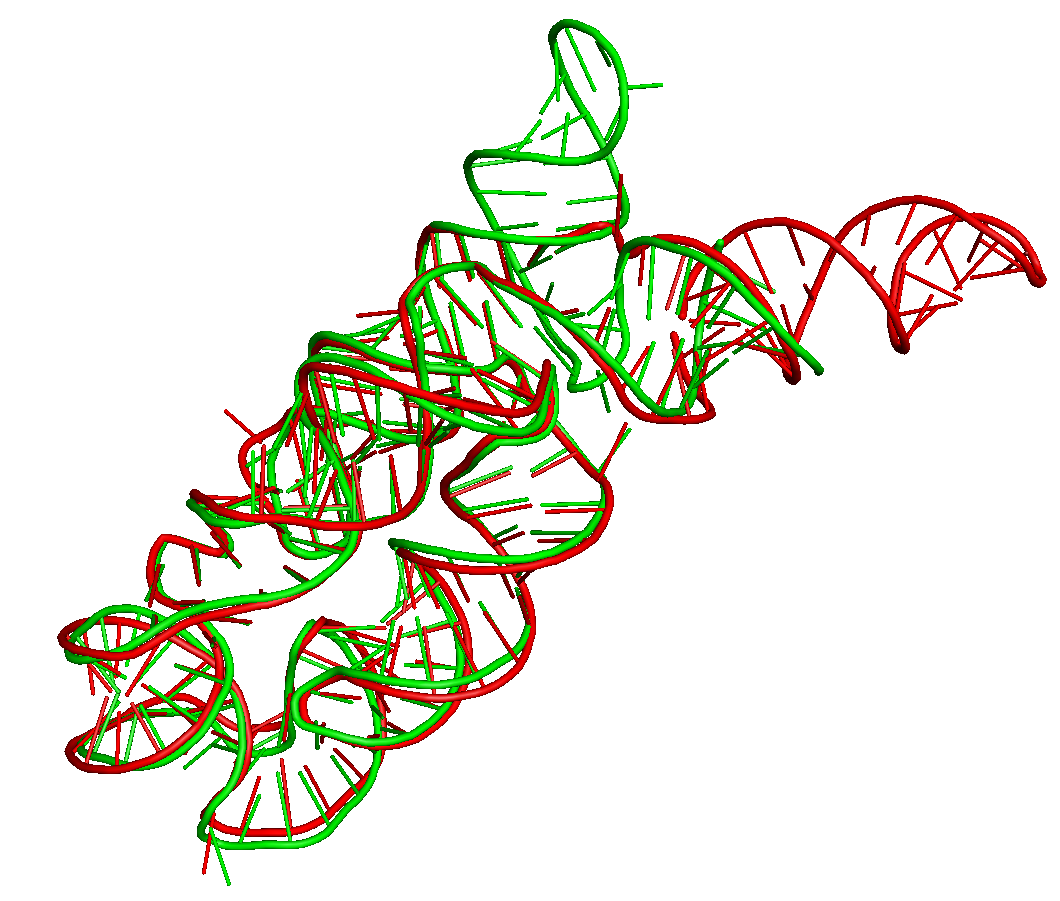
\includegraphics[width=\textwidth]{../img/badPredictedRegion}
\caption{Na obrázku vidíme zarovnanie experimenntálne získanej (3DIG) štruktúry a jej predikcie, napredikovanou našim algoritmom vytvoreným v bakalárskej práci. V pravej hornej časti obrázka vidíme, že algoritmu FARFAR sa nepodarilo správne napredikovať nekonzervovaný úsek.}
\label{obr3.3:badPredictedRegion}
\end{figure}
